\documentclass[a4paper,12pt,twoside]{article}

\setlength\oddsidemargin{-0.25cm}
\setlength\evensidemargin{-0.25cm}
\setlength\textwidth{15.0cm}
\addtolength{\voffset}{-40pt}
\addtolength{\textheight}{80pt}
\linespread{1.3}

\usepackage{amsthm}
\usepackage{array}
\usepackage{amsmath}
\usepackage{amssymb}
\usepackage{alltt}
\usepackage{graphicx}
\usepackage{url}
\usepackage{color,fancyvrb}
\usepackage{helvet}

\definecolor{myblue}{rgb}{0.2,0.6,1.0}


\theoremstyle{definition} \newtheorem{thm}{Theorem}
\theoremstyle{definition} \newtheorem{defn}{Definition}

\newcommand{\pic}{$\pi$-calculus}
\newcommand{\ba}{\begin{alltt}\small}
\newcommand{\ea}{\end{alltt}}
\newcommand{\bfns}{\begin{alltt}\footnotesize}
\newcommand{\efns}{\end{alltt}}
\newcommand{\cd}{\small \texttt}
\newcommand{\cdfns}{\fns \texttt}
\newcommand{\M}[1]{$\mathcal{#1}$}
\newcommand{\Mw}[1]{\mathcal{#1}}
\newcommand{\Initial}{\texttt{Initial}}
\newcommand{\Running}{\texttt{Running}}
\newcommand{\Completed}{\texttt{Completed}}
\newcommand{\Cancelled}{\texttt{Cancelled}}

\newcommand{\SCTT}{$\mathcal{M}\llbracket - \rrbracket$}
\newcommand{\SCTTTEM}{$\mathcal{M}_{template}\llbracket - \rrbracket$}
\newcommand{\SCTL}{$\mathcal{M}\llbracket$}
\newcommand{\SCTLTEM}{$\mathcal{M}_{template}\llbracket$}
\newcommand{\SCTR}{$\rrbracket$}
\newcommand{\STTT}{$ST$}
\newcommand{\CTTT}{$CT$}
\newcommand{\SCQTT}{$\mathcal{Q}\mathcal{T}\llbracket - \rrbracket$}
\newcommand{\SCQTL}{$\mathcal{Q}\mathcal{T}\llbracket$}
\newcommand{\SCQTR}{$\rrbracket$}
\newcommand{\CTT}{$\mathcal{C}\mathcal{T}\llbracket - \rrbracket$}
\newcommand{\CTL}{$\mathcal{C}\mathcal{T}\llbracket$}
\newcommand{\CTR}{$\rrbracket$}

\newcommand{\flow}{\texttt{$<$flow$>$}}
\newcommand{\pick}{\texttt{$<$pick$>$}}
\newcommand{\while}{\texttt{$<$while$>$}}
\newcommand{\ifs}{\texttt{$<$if$>$}}
\newcommand{\seq}{\texttt{$<$sequence$>$}}
\newcommand{\src}{\texttt{$<$source$>$}}
\newcommand{\tar}{\texttt{$<$target$>$}}
\newcommand{\tc}{\texttt{$<$transitionCondition$>$}}
\newcommand{\jc}{\texttt{$<$joinCondition$>$}}
\newcommand{\ru}{\texttt{$<$repeatUntil$>$}}
\newcommand{\fe}{\texttt{$<$forEach$>$}}
\newcommand{\ex}{\texttt{$<$exit$>$}}
\newcommand{\comp}{\texttt{$<$compensate$>$}}
\newcommand{\throw}{\texttt{$<$throw$>$}}
\newcommand{\rethrow}{\texttt{$<$rethrow$>$}}
\newcommand{\rec}{\texttt{$<$receive$>$}}
\newcommand{\rep}{\texttt{$<$reply$>$}}
\newcommand{\inv}{\texttt{$<$invoke$>$}}
\newcommand{\val}{\texttt{$<$validate$>$}}
\newcommand{\wait}{\texttt{$<$wait$>$}}
\newcommand{\empt}{\texttt{$<$empty$>$}}
\newcommand{\ass}{\texttt{$<$assign$>$}}
\newcommand\HRule{\noindent\rule{\linewidth}{1.5pt}}

\begin{document}
\begin{titlepage}
\vspace*{\stretch{1}}
\HRule
\begin{flushright}
\LARGE Model-based Orchestration \\
\large andrew.farrell@hp.com \\
\normalsize Last updated: 9th June 2008 \\
\LARGE Overview \\
\normalsize Version 1.2 (of this documentation)\\
(best printed in colour!)
\end{flushright}
\HRule
\vspace*{\stretch{2}}
\centering

\includegraphics[scale=0.4]{sflabsng}
\end{titlepage}

\cleardoublepage
\tableofcontents
\cleardoublepage
\section*{Change History}
\par\noindent 1.0 Initial tidy-up of original documentation  \cd{trunk/core/smartfrog/docs/SFOrchestration.pdf}
\par\noindent 1.1 Initial documentation for new engine  \cd{trunk/core/smartfrog/docs/SFOrchestration1\_1.pdf}
\par\noindent 1.2 Release documentation for new engine \cd{trunk/core/smartfrog/docs/SFOrchestration1\_2.pdf}

This document = Version 1.2

\cleardoublepage
\section{Introduction}

The purpose of the orchestration extension to SmartFrog is to provide a means by which the execution of logic within SmartFrog components may be orchestrated.

The fundamental concept is as follows.  An orchestration is a set of SmartFrog components.  Each component in the set defines dependencies which guard whether it may do some work and then change state.  For information regarding why this particular model of orchestration may prove beneficial over traditional workflow-based approaches to orchestration see \cite{R2D2}.

A very simple example is the following.  Let's say that there is a system of three managed entities, on which we wish to orchestrate management actions.  Each managed entity may be \cd{created} and subsequently \cd{removed}.  The initial state for each entity is that it is neither \cd{created} nor \cd{removed}.  Consider also that the second may not be \cd{created} until the first has been \cd{created}.  Similarly, the third may not be \cd{created} until the second has been \cd{created}. Conversely, the second may not be \cd{removed} until the third has been \cd{removed}.  Similarly, the first may not be \cd{removed} until the second has been \cd{removed}.  This orchestration is captured in Figure~\ref{Example1}.  

\begin{figure}[!h]
\centering
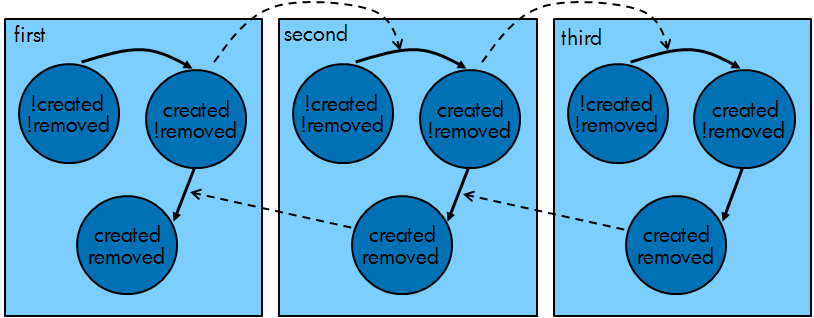
\includegraphics[scale=0.5]{cr}
\caption{A Simple Orchestration}\label{Example1}
\end{figure}

In the figure, there is for instance a dependency (dotted arrow) on \cd{second} for it to move from \cd{(!created,!removed)} to \cd{(created,!removed)} states that \cd{first}'s \cd{created} attribute is \cd{true}. 

\section*{Where To Find Stuff}
The new release of the orchestration engine is situated at:
\par \cd{org.smartfrog.services.dependencies}
\par\noindent within the open source release of SmartFrog at \cd{www.smartfrog.org}.

In order for the SmartFrog parser to perform verification of orchestration models, it is currently necessary to copy the appropriate \cd{NuSMV} dynamic library from \linebreak[4] \cd{trunk/core/extras/modelchecker/nusmv/lib} to \cd{SFHOME/lib/NuSMV}.  In time, this copy will be automated as part of the build process.  Copy \cd{NuSMVInterface.dll} if running SmartFrog under Win32 or \cd{libNuSMVInterface.so} if under Linux32.  Currently, we do not support verification of orchestrations for 64-bit operating systems.  

\cleardoublepage
\section{Language Overview}
\section*{Example Orchestration Model}

{\scriptsize
\begin{Verbatim}[frame=single, rulecolor=\color{myblue}, framerule=1pt, framesep=1pc]

#include "org/smartfrog/components.sf"
#include "org/smartfrog/services/dependencies/statemodel/components.sf"
#include "org/smartfrog/services/dependencies/threadpool/components.sf"

ManagedEntity extends State {
   sfClass "org.smartfrog.services.dependencies.examples.ManagedEntity";

   //Orchestration State 
   created false;
   removed false;
   //Non-orchestration State
   name TBD;
   
   tcreated extends Transition {       
      dependency (! LAZY created);
      statefunction extends {
          created true;
      }
   }
   tremoved extends Transition {
      dependency (LAZY created  && (! LAZY removed));
      statefunction extends {
          removed true;
      }
   }  
}

createdDependency extends Dependency {
   enabled LAZY on:created;
   relevant (! LAZY by:created);
}
removedDependency extends Dependency {
   enabled LAZY on:removed;
   relevant ((! LAZY by:removed) && LAZY by:created);
}
 
ManagedEntities extends Model {

   killMe extends CompositeTerminator {
   	  terminateCond LAZY foo0:removed;
   }

   foo0 extends ManagedEntity{
      name "foo0";
   }
   foo1 extends ManagedEntity{
      name "foo1";
   }
   foo2 extends ManagedEntity{
      name "foo2";
   }
   
   foo0Created extends createdDependency {
      on LAZY foo0;
      by LAZY foo1;
   }
   foo1Created extends createdDependency {
      on LAZY foo1;
      by LAZY foo2;
   }
   foo2Removed extends removedDependency {
      on LAZY foo2;
      by LAZY foo1;
   }
   foo1Removed extends removedDependency {
      on LAZY foo1;
      by LAZY foo0;
   }
   
   -- extends VerificationRecord {
   	  proposition "AG({foo0:created} -> {foo1:created})";
   }
}
\end{Verbatim}
}

\section*{Model}
As may be seen from the foregoing example, an orchestration model is specified as (a prototype) extending \cd{Model}.


\section*{State}
In the example, we define a component prototype called \cd{ManagedEntity} which extends the \cd{State} prototype defined in:  \cd{/org/smartfrog/services/dependencies/statemodel/components.sf}.  

{\scriptsize
\begin{Verbatim}[frame=single, rulecolor=\color{myblue}, framerule=1pt, framesep=1pc]
ManagedEntity extends State {
   sfClass "org.smartfrog.services.dependencies.examples.ManagedEntity";

   created false;
   removed false;
   name TBD;
   
   tcreated extends Transition {       
      dependency (! LAZY created);
      statefunction extends {
          created true;
      }
   }
   
   tremoved extends Transition {
      dependency (LAZY created  && (! LAZY removed));
      statefunction extends {
          removed true;
      }
   }  
}

\end{Verbatim}
}

A state component will list a number of transitions, which are prototype descriptions which extend \cd{Transition}.  It will also list a number of attributes that compose its ``working state''.  The working state of a state component is the sum of all of its attributes except its transitions.  The working state is itself divided into two disjoint sets: orchestration and non-orchestration state.  

The orchestration state of a component are those attributes whose values may only be changed in accordance with the transitions specified by the component.  Non-orchestration state may be changed arbitrarily.  Note that there is no tagging to indicate which is which - this information is inferred from the component description. 

In the example, we define two transitions: one which manipulates the value of the \cd{created} attribute, and another which manipulates the \cd{removed} attribute. Any transition can manipulate any subset of the orchestration state.  In this example, the orchestration state comprises \cd{removed} and \cd{created}.  The attribute \cd{name} comprises the non-orchestration state. 

\section*{Transition}
A transition expresses two things: a dependency proposition and a state function.

The dependency proposition specified within a transition is typically a dependency based on (a subset of) the orchestration state of the component specifying the given transition, although it need not be.  Whether a transition is applicable at any time will depend in part on its dependency proposition as well as other factors -- this is elaborated in \textit{Formal Specification of Semantics}.

In the example, \cd{tcreated}'s dependency proposition prescribes that the \cd{created} attribute of the \cd{ManagedEntity} be \cd{false}.

A state function expresses how attributes are to be updated.  It is a map of attributes for update against specifications of how to update them.  A specification may be some simple value literal, a reference, or a data description specifying alternative values for the attribute being set -- each attribute of the description specifying an alternative.  A reference may only (directly or indirectly) refer to the \textit{orchestration state} of the pertaining or other components. 

Examples of all of these possibilities are now given:
\begin{itemize}
\item Simple literal value

{\scriptsize
\begin{Verbatim}[frame=single, rulecolor=\color{myblue}, framerule=1pt, framesep=1pc]
statefunction extends {
   foo 2;
   foo2 12;
}
\end{Verbatim}
}

\item Reference (including an APPLY reference, specifying an expression)

{\scriptsize
\begin{Verbatim}[frame=single, rulecolor=\color{myblue}, framerule=1pt, framesep=1pc]

statefunction extends {
   foo LAZY bar;
   foo2 (LAZY bar1 + LAZY bar2);
}
\end{Verbatim}
}

\item Non-deterministic choice from alternatives.  Here, foo is assigned to either 2 or 12.

{\scriptsize
\begin{Verbatim}[frame=single, rulecolor=\color{myblue}, framerule=1pt, framesep=1pc]
statefunction extends {
   foo extends {
      -- 2;
      -- 12;
   }
}

\end{Verbatim}
}
\end{itemize}

The state function for \cd{tcreated} simply sets \cd{created} to \cd{true}, as can be seen in the previous presentation of the \cd{ManagedEntity} prototype.

\section*{External Dependencies}
In a model, we may specify a number of dependencies \textit{between} components, which we shall call \textit{external} dependencies.  These are in contrast to what we have described so far, namely dependencies \textit{within} components -- i.e. dependencies which guard when a transition is applicable for a component based on its current state. 

An external dependency constrains the behaviour of a component by specifying a condition which must (at least) hold for the component to change orchestration state.  The condition has a pair of propositions associated with it: \cd{relevant}, which determines when the condition applies, and \cd{enabled} - which prescribes when the condition is satisfied if relevant.

The general form for a dependency is:

{\scriptsize
\begin{Verbatim}[frame=single, rulecolor=\color{myblue}, framerule=1pt, framesep=1pc]
myDependency extends Dependency {
    on LAZY someReference;     // to a state component or connector
    by LAZY another Reference; // to a state component or connector
    relevant aLazyProprosition;
    enabled anotherLazyProposition;
    transition ``transition name'';  //optional, could also be a vector of strings
}
\end{Verbatim}
}

A dependency is considered to be satisfied just in the events that enabled is true or relevant is false (i.e. in propositional logic if \cd{relevant$\rightarrow$enabled} holds).

An example of a dependency from the presented orchestration model is:

{\scriptsize
\begin{Verbatim}[frame=single, rulecolor=\color{myblue}, framerule=1pt, framesep=1pc]
foo0Created extends createdDependency {
    on LAZY foo0;
    by LAZY foo1;
}
\end{Verbatim}
}

This is a dependency, as can be seen, between components \cd{foo0} and \cd{foo1}.  This prototype extends \cd{createdDependency} which defines values for \cd{relevant} and \cd{enabled}:

{\scriptsize
\begin{Verbatim}[frame=single, rulecolor=\color{myblue}, framerule=1pt, framesep=1pc]
createdDependency extends Dependency {
   enabled LAZY on:created;
   relevant (! LAZY by:created);
}
\end{Verbatim}
}

The values specified for these attributes means that the dependency is satisfied just in the events that foo0's \cd{created} attribute is \cd{true} or \cd{foo1}'s created attribute is \cd{true}.
The sum of dependencies specified for a component are implicitly subject to an AND-evaluation, meaning that for a component to be enabled all dependencies specified for it need to be satisfied.  

An external dependency as described so far is a condition on the enablement of the state component as a whole.  It can be made to be transition-specific through the inclusion of a \cd{transition} attribute.  This restricts the dependency condition to the named transition within the \textit{by} component.  Consider the following example.

{\scriptsize
\begin{Verbatim}[frame=single, rulecolor=\color{myblue}, framerule=1pt, framesep=1pc]
dep extends Dependency {
    on LAZY zoo0; 
    by LAZY zoo1; 
    relevant LAZY on:bar0;
    enabled LAZY on:bar1;
    transition "fred"
}
\end{Verbatim}
}

Just transition \cd{fred} within \cd{zoo1} is subject to this dependency.  If \cd{transition} were \cd{["fred", "bob"]}, then just ``fred'' and ``bob'' would be subject to the dependency.

\section*{Connector}
There are a number of \textit{connectors}: \cd{AndConnector}, \cd{OrConnector}, \cd{NandConnector}, \cd{NorConnector} and \cd{XorConnector}.  They aggregate dependencies according to the standard truth table semantics of AND, OR, NAND, NOR and XOR, respectively.  

Dependencies which name a connector in their \textit{by} attributes serve as the input dependencies for a connector.  For an AND connector, if all such dependencies are satisfied at any time, then the connector is enabled (i.e. satisfied).  For OR, just one such dependency needs to be satisfied.  All dependencies which name a connector in their \textit{on} attributes are enabled just when the connector is enabled and the evaluation of relevant$\rightarrow$enabled holds for the dependency.

\section*{Composite}
Composites aggregate other composites, state components, dependencies and connectors, serving to promote modularity in the definition of a model.  In this vein, they facilitate \textit{compositionality} by exposing an interface by which a composite may be connected to other orchestration artefacts to form a model.  

That is to say, the simplest way in which a fragment of one orchestration model may be reused in other or new models is for it to be bundled as a composite which enumerates a number of ports or connectors by which its behaviour may be influenced by the target model and vice-versa.  

Input connectors are used to wire dependencies into the composite so that the behaviour of the composite is influenced by that of the rest of the model.  Output connectors are used to wire dependencies out of the composite so that the behaviour of the rest of the model may be influenced by that of the composite.

From \cd{/org/smartfrog/services/dependencies/statemodel/components.sf}, the definition of a composite is as follows.

{\scriptsize
\begin{Verbatim}[frame=single, rulecolor=\color{myblue}, framerule=1pt, framesep=1pc]
Composite extends Compound {
     sfClass "org.smartfrog.services.dependencies.statemodel.state.Composite";
     sfUpdatable true;

     threadpool LAZY PROCESS:threadpool; // default place for the threadpool

     inputConnectors extends Compound {
        sfUpdatable true;
     }
     outputConnectors extends Compound {
        sfUpdatable true;     
     }
}
\end{Verbatim}
}

Here, we see the input and output connector \cd{Compound}s.  Connectors within these \cd{Compound}s are referred to by dependencies within/outside the composite.  The general form of extending a composite is as follows.

{\scriptsize
\begin{Verbatim}[frame=single, rulecolor=\color{myblue}, framerule=1pt, framesep=1pc]
myComposite extends Composite {
    inputConnectors:ic extends AndConnector;
    outputConnectors:oc extends AndConnector;

    s1 extends State { }
    s2 extends State { }
    c extends Composite { }

    d1 extends Dependency {
       on LAZY inputConnectors:ic;
       by LAZY s1;
    }
    d2 extends Dependency {
       on LAZY s2;
       by outputCOnnectors:oc;
    }

    etc
}
\end{Verbatim}
}

Note that a model is implemented as a \cd{Composite} (with no input/output connectors).

\section*{CompositeTerminator}
A composite may specify a \cd{CompositeTerminator} which has the effect of terminating the composite when the \cd{terminateCond} condition specified therein holds.  The single instance in the previous model was:

{\scriptsize
\begin{Verbatim}[frame=single, rulecolor=\color{myblue}, framerule=1pt, framesep=1pc]
   killMe extends CompositeTerminator {
   	  terminateCond LAZY foo0:removed;
   }
\end{Verbatim}
}

For the time being, a \cd{CompositeTerminator} may only be attached to a model.

\section*{Verification Record}
A verification record specifies a proposition in some temporal logic which must hold for the model when parsed.  See \textit{Verification} for more details.

\cleardoublepage
\section{Programming State Components}
State components are programmed as extensions of \newline \cd{org.smartfrog.services.dependencies.statemodel.ThreadedState}.

The \cd{ManagedEntity} prototype specified in the orchestration model previously specifies the following component class in its \cd{sfClass} attribute.

{\scriptsize
\begin{Verbatim}[frame=single, rulecolor=\color{myblue}, framerule=1pt, framesep=1pc]
package org.smartfrog.services.dependencies.examples;

import java.rmi.RemoteException;
import org.smartfrog.services.dependencies.statemodel.state.ThreadedState;
import org.smartfrog.sfcore.prim.Prim;

public class ManagedEntity extends ThreadedState implements Prim {
			
	public ManagedEntity() throws RemoteException {super();}  
	
	public boolean requireThread(){ return true; }  
	
	public boolean threadBody(){
		selectSingleAndGo();  //ignore return value...
		return true;
	}
}
\end{Verbatim}
}

Once a component is created and initialized (using the normal SF lifecycle), it will be invoked to do something as part of a notification cycle which fires whenever a transition is made within the orchestration model.

An invocation consists of the following two steps:
\begin{itemize}
\item The \cd{requireThread} method is called. As its name suggests, the method is called to determine whether a thread is needed for the purpose of carrying out the work needed to make a transition.  As an alternative, very light work may be carried out within the body of this method itself.  Note carefully, however, as this method is called within the notification cycle it is important to ensure timely completion of its execution. 

The method returns \cd{true} if the component determines that a separate thread is needed to make a transition, and \cd{false} otherwise.  It may also return \cd{false} if no transition is to be made, in which case the component remains in its current orchestration state.

\cd{requireThread} may also be used to determine whether a transition which has previously been scheduled for a component, but which is yet to be carried out, should be removed.  If it is not to be removed, then we would return \cd{false}.  If it should be removed, then we return \cd{true}.  It is not possible to remove a thread if it has been started already.  In this case, the \cd{requireThread} method would not get called in the first place, as the currently running transition would be allowed to complete.

\item If a separate thread is required, we implement the logic to be run inside the \cd{threadBody} method. The thread body will be placed on a thread pool queue for execution as soon as a thread becomes free.  Note that a \cd{threadBody} also returns a value. This pertains to whether the transition should be considered to be complete when the \cd{threadBody} returns (synchronous behaviour), or whether it will complete at a later time (asynchronous behaviour).  We will come back to this point later.
\end{itemize}

There are a number of methods available within \newline \cd{org.smartfrog.services.dependencies.statemodel.State} which allow access and manipulation of orchestration and non-orchestration state from within \cd{requireThread} and \cd{threadBody}.
\begin{itemize}
\item \cd{HashMap<String, Object> getLocalOrchestrationState()}, \linebreak[4] 
\cd{HashMap<String, Object> getLocalNonOrchestrationState()}, \linebreak[4] 
\cd{HashMap<String, Object> getLocalState()}, 
\par These methods make the local orchestration / non-orchestration state of the component available for inspection.  Note that these are clones so changes made to the returned context will have no effect on component state.  
\item \cd{HashMap<String, ComponentDescription> getPossibleTransitions() \linebreak[4] 
throws StateComponentSetAttributException} 
\par Returns a hashmap of the currently enabled transitions for the component.  
\item \cd{void setTransitionToCommit(String transition\_name) \linebreak[4]
throws StateComponentSetAttributException} 
\par Having studied the possible transitions returned by the previous method, one of them may be selected for initiation.   If no such transition is available for selection, the given exception is thrown.
\item \cd{void setAttribute(String key, Object value) \linebreak[4] throws StateComponentSetAttributException} 
\par Used to set an attribute of non/orchestration state.  For orchestration state, it only may be used for attributes whose state function determines that there is a choice of values that may be assigned. 
\item \cd{void go() throws StateComponentSetAttributException} 
\par Commit changes specified in calling \cd{setAttribute}
\item \cd{boolean selectSingleAndGo()} \linebreak[4]
\par May be used when there is a single transition applicable to a component - will return \cd{false} otherwise - with deterministic next values for attributes (according to the transition).  That is, it does a select of transition (\cd{setTransitionToCommit}) and \cd{go()} all in one.
\end{itemize}

In the example, the dependencies are structured such that whenever a component is enabled, it will have a transition that it can make.  Moreover, because in any particular instance there is only one transition that is applicable and its state function deterministically prescribes the next values of the pertinent attributes, we may simply call \cd{selectSingleAndGo()} in order to effect the given transition.  In all of the managed entities, the first applicable transition is to set \cd{created} to \cd{true}, the second is to set \cd{removed} to \cd{true}. 

Continuing with the example, the \cd{threadBody} completes its appropriate action by the time it returns.  This is indicated by the fact that it returns \cd{true}.   This characteristic is fine unless a state component interacts with some external entity that can take a long time to complete -- for example waiting for a server to boot which can take several minutes. This would simply block a thread from the thread pool and limits parallelism. For these cases, the \cd{threadBody} can choose to complete asynchronously.  

To complete asynchronously, the \cd{threadBody} returns the value \cd{false} to indicate non-completion. Through some internal mechanism or a call-back by some 3rd party code, an appropriate transition may be subsequently made to the component using the API methods presented above.   Having returned \cd{false} from \cd{threadBody}, no further action is possible within the component whilst the asynchronous action is yet-to-complete.

There are times when completely asynchronous events occur - for example a part of the state that is managed by the state component fails, an internal timer fired, or some external management entity wants to force an action from the state component.   In this case, the management (or other) logic must implement the callback interface: 
\cd{org.smartfrog.services.dependencies.statemodel.InvokeAsynchronousStateChange}.

This has a single method: 
\cd{public void actOn(State sc)}

The body of an implementation of this method constitutes the desired management logic.  It may make full use of the API just presented in order to effect a transition for a component.

There is an additional method in \cd{State}, which when called causes the \cd{actOn} method to be called:
\cd{public void invokeAsyncStateChange(InvokeAsynchronousStateChange iasc)
throws StateComponentSetAttributException}

We pass the object implementing \cd{InvokeAsynchronousStateChange} which has the desired implementation of management logic, as shown:

{\scriptsize
\begin{Verbatim}[frame=single, rulecolor=\color{myblue}, framerule=1pt, framesep=1pc]
   public void managementMethod(...) {
       //whatever code

	comp.invokeAsyncStateChange(new InvokeAsynchronousStateChange(){
	     public void actOn(State _comp) {
		    HashMap<String,ComponentDescription> possible =
 						_comp.getPossibleTransitions();
  		    ...	
             }
	}
   }
\end{Verbatim}
}

\section*{Thread Pool}
For the orchestration engine to work it relies on a threadpool being available on each host.  There are currently two SmartFrog configuration descriptions made available for thread pools.   One uses the \cd{java.util.concurrent} functionality available since Java 1.5, and the other uses our own implementation.  

There is not a great deal to choose between them for our purposes. The former description is located thus: \cd{org/smartfrog/services/dependencies/threadpool/simpletp.sf}.  The latter is located at: \cd{org/smartfrog/services/dependencies/threadpool/threadpool.sf}.  

\cleardoublepage
\section{Formal Specification of Semantics}
In this section, we introduce a formal account of the semantics of our orchestration approach.  We divide the presentation into two parts.  Firstly, we give a simplified account which enables the reader to get to the nub of the semantic characterisation.  We then give an account which is much closer to the way in which the orchestration engine that we have implemented works, and which is much closer to what is exposed to a model author through the authoring front-end which has been implemented in this work.  

The purpose of this second account is to give a precise crystallisation of the semantics of our modelling approach. The principal difference between the two accounts is that second account more readily facilitates compositionality of orchestration fragments. Interestingly, the second account can be shown to not add anything extra in expressivity, and any model expressed using the second account may be mapped to a model using the first account.  Note that some model structure is lost in such a mapping meaning that, once mapped, it is not possible to perform a reverse mapping.

We start the presentation with some preliminaries before describing the two accounts of our orchestration approach.

\subsection*{Primitive Sets}
We assume a number of \textit{primitive sets}, which are pre-defined sets of primitive objects:
\begin{itemize} 
\item \cd{Strings} -- the set of all string literals.
\item \cd{Boolean} -- \{\cd{true}, \cd{false}\}.
\item \cd{Number} -- the set of all numbers. 
\end{itemize}

We also define \cd{Object}, which is a universal set -- the union of all primitive sets.  

\subsection*{Non-primitive Sets}
We also define the following non-primitive sets. 
\begin{itemize}
\item \M{C} -- the set of \textit{components} used in a model.  
\item \M{P} -- the set of \textit{composites} used in a model.  
\item \M{D} -- the set of all \textit{dependencies} possible in a model.  
It is the smallest set for a model \cd{$p$} containing:
\begin{itemize}
\item \cd{true} and \cd{false} 
\item \cd{($t$,$k$,$v$)} if \cd{$c_{t} \in \Mw{C}$ $\wedge$ $\exists m$,$T.c_{t}$=($t$,$m$,$T$) $\wedge$ $\exists v'$.map\_get($m$,$k$)=$v'$ $\wedge$ $v\in$Object} holds
\par (Every key in each component may be used in a dependency with any value from \cd{Object})

\item \cd{($d'$ \& $d''$)} if \cd{$d'$} and \cd{$d''$} are also in \cd{\M{D}} 
\item \cd{($d'$ | $d''$)} if \cd{$d'$} and \cd{$d''$} are also in \cd{\M{D}} 
\item \cd{($d'$ $\rightarrow$ $d''$)} if \cd{$d'$} and \cd{$d''$} are also in \cd{\M{D}} 
\item \cd{($d'$ $\leftrightarrow$ $d''$)} if \cd{$d'$} and \cd{$d''$} are also in \cd{\M{D}} 
\item \cd{!$d'$} if \cd{$d'$} is also in \cd{\M{D}}
\end{itemize}

\item \M{SF} -- the set of all \textit{state functions} possible in a model.  Each state function given a \textit{map} of ($key$,$value$) pairs will yield a new map whose set of keys is identical, but whose values may have changed. That is, for a map $m$ and any state function $sf$:
\par \cd{$\forall k$.($\exists v$.map\_get($m$,$k$)=$v$ $\equiv$ $\exists v'$.map\_get($sf$($m$),$k$)=$v'$)}
\end{itemize}

\subsection*{Auxiliary Functions and Predicates}
In the following, we introduce model artefacts such as composites and components.  There are a number of auxiliary functions and predicates that are used in this account. 
\begin{itemize}
\item We make use of a \textit{map} abstraction, which stores (key,value) pairs. 
\par \cd{map\_get($m$,$k$)=$v$} -- gets the value $v$ for key $k$ from map $m$

\item For composites: 
\par \cd{composite($n$,$p$)=$q$} extracts the composite $q$ with name $n$ from composite $p$

\item For components: 
\par \cd{component($n$,$p$)=$c$} extracts the component $c$ with name $n$ from composite $p$
\item For dependencies:
\par \cd{satisfied($d$,$p$)} determines whether (internal) dependency $d$ is satisfied in the context of model $p$
\par \cd{satisfied($d$,$t$,$c$,$p$)} determines whether transition $t$ is enabled in component $c$ according to internal dependency $d$ against model $p$ and any external dependencies that may exist in $p$
\end{itemize}

\cleardoublepage
\subsection*{Account I Semantics}
We present the first (i.e. simplified) account of the semantics for model-based orchestration.  For convenience, we introduce the structure of a model as we go along rather than separately. 

\subsection*{Model}
A \textit{model} is a triple: \cd{(\M{C},\M{D},\M{SF})}, that is, a set of components, a set of possible dependencies and a set of possible state functions.  For simplicity, in the following we refer to \M{C},\M{D}, and \M{SF} explicitly. 

Models are ranged over by $p$,$p'$,$\ldots$.

\subsection*{Component}
A \textit{component} is a triple: \cd{($n$,$m$,$T$)}, such that:
\begin{itemize}
\item \cd{$n$} is a name (from \cd{Object}) for the component which is unique wrt other components within the model
\item $m$ is a map, which stores (key,value) pairs
\item \cd{$T\subseteq$\M{T}} is a set of \textit{state transitions}, where \cd{\M{T}=Object$\times \Mw{D}\times$\M{SF}$\times$Boolean}, where:  

\begin{itemize}
\item The \cd{Object} value used in a state transition is a name for it that is unique within \cd{$T$} of which it is a member. 
\item The \cd{Boolean} value used in state transitions indicates whether the transition has been initiated but not yet finished or committed (indicated by \cd{true}), or not (indicated by \cd{false}).  Initially, this is always set to \cd{false}.
\end{itemize}
\end{itemize}

Components are ranged over by $c$,$c'$,$\ldots$ and sets thereof by $C$,$C'$$,\ldots$.  Dependencies are ranged over by $d$,$d'$,$\ldots$, and sets thereof by $D$,$D'$,$\ldots$. State transitions are ranged over by $t$,$t'$,$\ldots$ and sets thereof by $T$,$T'$,$\ldots$.  State functions are ranged over by $sf$,$sf'$,$\ldots$.

The auxiliary function \cd{component} is characterised thus.  For a model $p$, comprising the set of components \M{C}, 
\par \cd{component($n$,$p$)=$c$ $\equiv$ $\exists m$,$T$.$c\in\Mw{C}$ $\wedge$ $c$=($n$,$m$,$T$)} 
\par (Holds when $c$ is a component of name $n$ within model $p$.)

\subsection*{Step System for a Model}
In the following, we characterise the behaviour of an orchestration model as a \textit{step system}.  This is similar in concept to a transition system, which is a common term, except that we reserve the term transition for state transitions.  A state transition is a pair of steps -- an initiating step where a particular state transition is chosen for a component but is yet-to-be-committed, and a committing/aborting step where the state transition may be either committed or aborted. If committed, the appropriate change in state occurs.  The relation \cd{$\rightarrow^{p}$} defines individual steps (that is, initiating and committing/aborting steps).

The step system \cd{$\rightarrow^{p}$} entailed by a model $p$ is the smallest set of pairs containing:
\begin{itemize}
\item \cd{($p$,$p'$)} if the relation \cd{Step($p$,$p'$)} holds, and $p'$ is a \textit{initial} model. (An initial model is a model which has been correctly initialised.  This means that the \cd{Boolean} value in state transitions, pertaining to whether the transition has been initiated, is universally set to \cd{false} for all transitions.)

\par (This characterises steps from the initial state.) 
\item \cd{($p''$,$p'$)} if \cd{($p$,$p''$)} is also in \cd{$\rightarrow^{m}$} and \cd{Step($p''$,$p'$)} holds
\par (This characterises steps from other states.)
\end{itemize}
where:

\begin{itemize}

\item \cd{Step($p$,$p'$) $\equiv$} 
\par \hspace{0.5cm} \cd{$\exists n$.($\exists c$,$c'$.component($n$,$p$)=$c$ $\wedge$ StepComponent($p$,$c$,$c'$) $\wedge$ component($n$,$p')=c'$)}
\par \hspace{0.5cm} (Step in one of the components)
\par \hspace{0.25cm} \cd{$\wedge$}
\par \hspace{0.5cm} \cd{$\forall n'$,$c''$.$n'\neq n \supset$ (component($n'$,$p$)=$c''$ $\equiv$ component($n'$,$p'$)=$c''$))}
\par \hspace{0.5cm} (No Expansion, and other components are identical)

\item \cd{StepComponent($p$,$c$,$c'$) $\equiv$ StepCommit($c$,$c'$) $\vee$ StepInitiate($p$,$c$,$c'$)}
\par (Either a committing or initiating step in a component.)

\item \cd{StepCommit($c$,$c'$) $\equiv$}
\par \hspace{0.5cm} \cd{$\exists d$,$sf$,$n$,$n'$,$m$,$m'$,$T$,$T'$.$c$=($n$,$m$,$T$) $\wedge$ $c'$=($n$,$m'$,$T'$) $\wedge$ ($n'$,$d$,$sf$,true)$\in T$ $\wedge$} 
\par \hspace{0.5cm} \cd{($m'$=$sf$($m$) $\vee$ $m'$=$m$)}
\par \hspace{0.5cm} (get new map by applying state function. We may abort the transition meaning that we offer the possibility of not making any changes)
\par \hspace{0.25cm} \cd{$\wedge$}
\par \hspace{0.5cm} \cd{$\forall n''$,$d'$,$sf'$,$b$,$b'$.(($n''$,$d'$,$sf'$,$b$) $\in$ $T$ $\wedge$ $b'$=false $\equiv$ ($n''$,$d'$,$sf'$,$b'$) in $T'$)}
\par \hspace{0.5cm} (get new set of transitions -- all \cd{false} regarding being initiating steps) 

%% If NEW then OLD with bnew as FALSE  (no additional transitions)
%% If OLD (and bnew is FALSE) then NEW   (no lost transitions)


\item \cd{StepInitiate($p$,$c$,$c'$) $\equiv$} 
\par \hspace{0.5cm} \cd{$\exists d$,$sf$,$n$,$n'$,$m$,$T$,$T'$.$c$=($n$,$m$,$T$) $\wedge$ $c'$=($n$,$m$,$T'$) $\wedge$ ($n'$,$d$,$sf,$false)$\in T$ $\wedge$ satisfied($d$,$p$) $\wedge$}
\par \hspace{0.5cm} \cd{$\forall n''$,$d'$,$sf'$,$b$,$b'$.}
\par \hspace{1.0cm} \cd{(($n''$,$d'$,$sf'$,$b'$)$\in T'$ $\supset$ ($n''$,$d'$,$sf$,$b$)$\in T$ $\wedge$ ($n'$=$n''$ $\wedge$ $b'$=true $\vee$ $n'\neq n''$ $\wedge$ $b'$=false) $\wedge$} 

\par \hspace{1.25cm} \cd{($n''$,$d'$,$sf$,$b$)$\in T$ $\supset$ ($n''$,$d'$,$sf'$,$b'$)$\in T'$ $\wedge$ $b$=false)} 
\par \hspace{0.5cm} (For an initiating step, check dependency and set boolean indicating `initiated' to true for particular state transition.)

%% IF NEW then OLD with specific bnew as TRUE and rest bnew FALSE
%% IF OLD then NEW with bold as FALSE

\end{itemize}

The auxiliary predicate \cd{satisfied($d$,$p$} is characterised as follows, for dependency $d$ and model $p$.

\par \cd{satisfied($d$,$p$) $\equiv$ $d$=true $\vee$}
\par \hspace{1cm} (Satisfied when \cd{$d$} is simply true or)
\par \hspace{0.75cm} \cd{$\exists d'$.$d$=!$d'$ $\wedge$ $\neg$satisfied($d'$,$p$) $\vee$}
\par \hspace{1cm} (Satisfied when \cd{$d$} is contingent on \cd{$d'$} being false and it is so or)
\par \hspace{0.75cm} \cd{$\exists d'$,$d''$.$d$=$d'$\&$d''$ $\wedge$ satisfied($d'$,$p$) $\wedge$ satisfied($d''$,$p$) $\vee$} 
\par \hspace{1cm} (Satisfied when \cd{$d$} is contingent on \cd{$d'$} and \cd{$d''$} being true and they are so or)
\par \hspace{0.75cm} \cd{$\exists d'$,$d''$.$d$=$d'$|$d''$ $\wedge$ (satisfied($d'$,$p$) $\vee$ satisfied($d''$,$p$)) $\vee$} 
\par \hspace{1cm} (Satisfied when $d$ is contingent on $d'$ or $d''$ being true and one of them is so or)
\par \hspace{0.75cm} \cd{$\exists d'$,$d''$.$d$=$d'\rightarrow d''$ $\wedge$ ($\neg$satisfied($d'$,$p$) $\vee$ satisfied($d''$,$p$)) $\vee$} 
\par \hspace{1cm} (Satisfied when \cd{$d$} is contingent on \cd{!$d'$} or \cd{$d''$} being true and one of them is so or)
\par \hspace{0.75cm} \cd{$\exists d'$,$d''$.$d$=$d'\leftrightarrow d''$ $\wedge$ (satisfied($d'$,$p$) $\wedge$ satisfied($d''$,$p$) $\vee$ $\neg$satisfied($d'$,$p$) $\wedge$ $\neg$satisfied($d''$,$p$)) $\vee$} 
\par \hspace{1cm} (Satisfied when \cd{$d$} is contingent on \cd{$d'$} and \cd{$d''$} both being true or both false and one is so or)
\par \hspace{0.75cm} \cd{$\exists n$,$k$,$v$,$m$,$T$.$d$=($t$,$k$,$v$) $\wedge$ component($t$,$p$)=($t$,$m$,$T$) $\wedge$ map\_get($m$,$k$)=$v$}
\par \hspace{1cm} (Satisfied when $d$ is a triple \cd{($t$,$k$,$v$)} and the key-value map for component with name $t$ 
\par \hspace{1cm} in model $p$ has a value of $v$ for key $k$)

\cleardoublepage
\subsection*{Account II Semantics}
In the second account, we add a little more structure to the modelling language and its characterisation.  We introduce the following further artefacts: composites, external dependencies and connectors. 

\subsection*{Model}
We now define a model to be a pair ($p$, \M{A}) where:
\begin{itemize}
\item $p$ is a composite (see below) which contains the orchestration model
\item \M{A} is an aggregation of artefacts used in the orchestration model. It is a quintuple: \cd{(\M{C},\M{P},\M{E},\M{D},\M{SF})} where:
\begin{itemize}
\item \M{C}, \M{D} and \M{SF} are (resp.) the set of components used, the set of (possible) dependencies, and the set of (possible) state functions, in the model (as previously described)
\item \M{P} is the set of composites used in the model
\item \M{E} is the set of external dependencies used in the model
\end{itemize}
\end{itemize}

In essence, then, a \textit{model} is a (single) composite, as shown in Figure~\ref{Model}.  
As will be described a composite itself contains a number of composites and components.

The model composite is now ranged over by $p$,$p'$,$\ldots$.  

For convenience, in the following narrative, we will refer to a model composite simply as a model, and refer to the constituents of \M{A} (namely, \M{C}, \M{D}, \M{SF}, \M{P}, and \M{E}), directly -- i.e., without reference to their containing model.

\subsection*{Component}
A \textit{component} is now a quadruple: \cd{($n$,$m$,$ac$,\M{T})}, where the additional member $ac$ of the tuple is a \cd{Boolean} value which determines whether the component may masquerade as an \textit{and connector} for the purposes of dependency evaluation.  

\begin{figure}
\centering
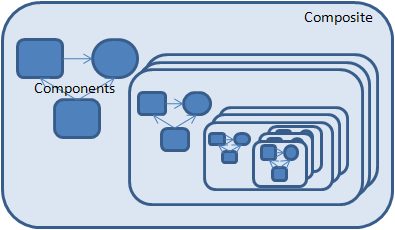
\includegraphics[scale=0.65]{cc}
\caption{An Orchestration Model}\label{Model}
\end{figure}

\subsection*{Composite}
A \textit{composite} is a quintuple: \cd{($n$,$P$,$C$,$IR$,$OR$)}, where:
\begin{itemize}
\item $n$ is a name (from \cd{Object}) for the composite which is unique wrt the set of composites within a model.
\item \cd{$P$} is a set of composites. 
\item \cd{$C$} is a set of components. 
\item \cd{$IR$} is a set of input connectors.
\item \cd{$OR$} is a set of output connectors.
\end{itemize}

Composites are ranged over by $p$,$p'$,$\ldots$,$q$,$q'$,$\ldots$.  Sets of composites are ranged over by $P$,$P'$,$\ldots$,$Q$,$Q'$,$\ldots$.

The auxiliary function \cd{composite} is thus characterised. For a model composite $p$ with associated set of composites \M{P}:
\par \cd{composite($n,p$)=$q$ $\equiv$ $\exists P$,$C$,$IR$,$OR$.$q\in\Mw{P}$ $\wedge$ $q$=($n$,$P$,$C$,$IR$,$OR$)} 
\par (Holds when $q$ is a composite of name $n$ within model $p$.)

\subsection*{External Dependency}
An \textit{external dependency} is a sextuple: \cd{($n$,$on$,$by$,$r$,$e$,$TN$)}, where:
\begin{itemize}
\item $n$ is a unique name (from \cd{Object}) for the dependency
\item $on$ is the name of an artefact (component or composite) within $p$
\item $by$ is the name of an artefact (component or composite) within $p$
\item $relevant$ is a dependency proposition (see previously) which may only refer to target attribute values which are part of the orchestration state within the \textit{on} and \textit{by} artefacts
\item $enabled$ is a dependency proposition with the same restriction as $relevant$
\item $TN$ is a set of transition names (can be empty) which constrain the applicability of the dependency to certain transitions of $by$ (if it is a state component).  If empty, the dependency is applicable to all transitions of $by$ (if a state component).
\end{itemize}

\subsection*{Connector}
A connector is simply one of \textit{and}, \textit{or}, \textit{nand}, \textit{nor}, and \textit{xor}.

\subsection*{Step System for a Model}
The definition of the step system for an Account II model is the same as that for Account I, with the exception of the definition of \cd{StepInitiate($p$,$c$,$c'$)}, which is now presented.  Moreover, the only change is the replacement of (the use of) \cd{satisfied($d$,$p$)} by (the use of) \cd{satisfied($d$,$t$,$c$,$p$)} (where, for $c$ read $n$ and for $t$ read $n'$).  

\par\vspace{0.5cm}
\par \cd{StepInitiate($p$,$c$,$c'$) $\equiv$} 
\par \hspace{0.5cm} \cd{$\exists d$,$sf$,$n$,$n'$,$m$,$T$,$T'$.$c$=($n$,$m$,$T$) $\wedge$ $c'$=($n$,$m$,$T'$) $\wedge$ ($n'$,$d$,$sf,$false)$\in T$ $\wedge$}
\par \cd{satisfied($d$,$n'$,$n$,$p$) $\wedge$}
\par \hspace{0.5cm} \cd{$\forall n''$,$d'$,$sf'$,$b$,$b'$.}
\par \hspace{1.0cm} \cd{(($n''$,$d'$,$sf'$,$b'$)$\in T'$ $\supset$ ($n''$,$d'$,$sf$,$b$)$\in T$ $\wedge$ ($n'$=$n''$ $\wedge$ $b'$=true $\vee$ $n'\neq n''$ $\wedge$}
\par \cd{$b'$=false) $\wedge$} 

\par \hspace{1.25cm} \cd{($n''$,$d'$,$sf$,$b$)$\in T$ $\supset$ ($n''$,$d'$,$sf'$,$b'$)$\in T'$ $\wedge$ $b$=false)} 
\par \hspace{0.5cm} (For an initiating step, check dependency and set boolean indicating `initiated' to true for particular state transition.)
\par\vspace{0.5cm}

\par The auxiliary predicate \cd{satisfied($d$,$t$,$c$,$p$)} is characterised as follows, for dependency $d$, transition $t$, component $c$ and model $p$.
\par\vspace{0.5cm}
\par\cd{satisfied($d$,$t$,$c$,$p$) $\equiv$ satisified($d$,$p$) $\wedge$ satisfied\_trans($t$,$c$,$p$)}
\par (A transition's dependency is satisfied iff the internal dependency is satisfied and any external dependencies for the pertaining component are also.)
\par\vspace{0.5cm}
\par\cd{satisfied\_trans($t$,$c$,$p$) $\equiv$}
\par (A component's external dependency is satisfied iff...)
\par {\small (nb: the ``\cd{trans}'' refers to the transition in question being taken into account -- see note below)}
\par\hspace{0.75cm}\cd{satisfied\_trans\_noapp($t$,$c$,$p$) $\vee$}
\par\hspace{1cm} (There is no applicable external dependency or)
\par\hspace{0.75cm} \cd{$\forall ed\in \Mw{E}$.$\exists o$,$r$,$e$,$T$.($ed$=($o$,$c$,$r$,$e$,$T$) $\wedge$ ($T=\emptyset$ $\vee$ $t \in T$) $\supset$ satisfied\_ed($ed$,$p$))}
\par\hspace{1cm} (All applicable dependencies -- i.e. those which name the transition in question, or whose set of pertinent transitions is empty -- are satisfied.)
\par\vspace{0.5cm}
\par\cd{satisfied\_trans\_noapp($t$,$c$,$p$) $\equiv$}
\par\hspace{0.75cm}\cd{$\forall ed \in \Mw{E}$.$\exists o$,$r$,$e$,$T$.($ed$=($o$,$c$,$r$,$e$,$T$) $\supset$ $\neg T=\emptyset \wedge \neg t \in T$)}
\par\hspace{1cm} (There is no applicable transition iff all external dependencies which name the component in their \textit{by} attribute have a non-empty $T$ -- they name specific transitions which scope the dependencies -- and the to-be-performed transition is not in any of the $T$s.)\par
\par\vspace{0.5cm}
\par\cd{satisfied\_ed($ed$,$p$) $\equiv$ $\exists o$,$b$,$r$,$e$,$T$.$ed$=($o$,$b$,$r$,$e$,$T$) $\wedge$}
\par\hspace{1cm} (An external dependency is satisfied iff)
\par\hspace{0.75cm}\cd{(($o \in \Mw{C} \wedge \exists on$,$om$,$oac$,$oT$.$o$=($on$,$om$,$oac$,$oT$) $\wedge$}
\par\hspace{0.9cm}\cd{$oac$=true $\vee$ $\neg o \in \Mw{C}$) $\supset$ satisfied\_notrans($o$,$p$)) $\wedge$}
\par\hspace{1cm} (If \textit{on} is a connector or a component masquerading as an andConnector then it must be enabled/satisfied and)
\par\hspace{0.75cm} \cd{(satisfied($r$,$p$) $\supset$ satisfied($e$,$p$))}
\par\hspace{1cm} (relevant$\rightarrow$enabled holds for the dependency)
\par\vspace{0.5cm}
\par\cd{satisfied\_notrans($c$,$p$) $\equiv$}
\par\hspace{1cm} (An \textit{on} component/connector is enabled/satisfied iff...)
\par\hspace{0.75cm}\cd{satisfied\_notrans\_noapp($c$,$p$) $\vee$}
\par\hspace{1cm} (There is no applicable external dependency or)
\par \hspace{0.75cm} \cd{($c\in \Mw{C}$ $\vee$ $c$=$and$) $\wedge$ satisfied\_notrans\_and($c$,$p$) $\vee$}
\par \hspace{1cm} (It is an andConnector or a component masquerading as one, and ... holds, or)
\par \hspace{0.75cm} \cd{$c$=$or$ $\wedge$ satisfied\_notrans\_or($c$,$p$) $\vee$}
\par \hspace{1cm} (It is an orConnector and ... holds, or)
\par \hspace{0.75cm} \cd{$c$=$nand$ $\wedge$ $\neg$satisfied\_notrans\_and($c$,$p$) $\vee$}
\par \hspace{1cm} (It is a nandConnector and the condition for an andConnector does not hold, or)
\par \hspace{0.75cm} \cd{$c$=$nor$ $\wedge$ $\neg$satisfied\_notrans\_or($c$,$p$) $\vee$}
\par \hspace{1cm} (It is a norConnector and the condition for an orConnector does not hold, or)
\par \hspace{0.75cm} \cd{$c$=$xor$ $\wedge$ $\exists ed\in \Mw{E}$,$o$,$r$,$e$,$T$.}
\par \hspace{1cm} (It is an xorConnector and)
\par \hspace{0.75cm} \cd{($ed$=($o$,$c$,$r$,$e$,$T$) $\wedge$ $T$=$\emptyset$ $\wedge$ satisfied\_ed($ed$,$p$) $\wedge$}
\par \hspace{1cm} (the condition for an orConnector holds, but...)
\par \hspace{0.75cm} \cd{$\forall ed'\in \Mw{E}$.$\exists o'$,$r'$,$e'$,$T'$($ed'$=($o'$,$c$,$r'$,$e'$,$T'$) $\wedge$ $T'$=$\emptyset$ $\wedge$ satisfied\_ed($ed$,$p$) $\supset$ $ed$=$ed'$)}
\par \hspace{1cm} (just one $T=\emptyset$ external dependencies may be satisfied)
\par \vspace{0.5cm}
\par\cd{satisfied\_notrans\_noapp($c$,$p$) $\equiv$}
\par\hspace{0.75cm}\cd{$\forall ed \in \Mw{E}$.$\exists o$,$r$,$e$,$T$.($ed$=($o$,$c$,$r$,$e$,$T$) $\supset$ $\neg T=\emptyset$)}
\par\hspace{1cm} (There is no applicable transition iff all external dependencies which name the component in their \textit{by} attribute have a non-empty $T$)
\par \vspace{0.5cm}
\par\cd{satisfied\_notrans\_and($c$,$p$) $\equiv$}
\par\hspace{0.75cm}\cd{$\forall ed\in \Mw{E}$.$\exists o$,$r$,$e$,$T$.($ed$=($o$,$c$,$r$,$e$,$T$) $\wedge$ $T=\emptyset$ $\supset$ satisfied\_ed($ed$,$p$))}
\par\hspace{1.0cm}(All $T=\emptyset$ external dependencies are satisfied.)
\par \vspace{0.5cm}
\par\cd{satisfied\_notrans\_or($c$,$p$) $\equiv$}
\par\hspace{0.75cm}\cd{$\exists ed\in \Mw{E}$,$o$,$r$,$e$,$T$.($ed$=($o$,$c$,$r$,$e$,$T$) $\wedge$ $T$=$\emptyset$ $\wedge$ satisfied\_ed($ed$,$p$))}
\par\hspace{1.0cm}(At least one of the component's $T=\emptyset$ external dependencies is satisfied.)
\par\vspace{1cm}
\par Note regarding \cd{satisified\_trans*} and \cd{satisfied\_notrans}:
\par When we assess the external enablement of a transition, each of the immediate dependencies for the transition may be (i) transition-specific, or (ii) non-transition-specific.  We take into account both for immediate dependencies, hence the use of \cd{satisified\_trans*} predicates.  Thereafter, when we ``follow'' dependencies, through their \cd{on} specifiers, we only take into account non-transition-specific external dependencies, hence the use of \cd{satisfied\_notrans*} predicates.

\section*{Termination}
In both semantic accounts, we may also specify a characterisation of termination.  That is, for a particular model, if any condition of a \cd{CompositeTerminator} for the model holds, then the model gets terminated.

To this end, we refine the definition of a model as follows.  Note that, we present a characterisation of the second account of our orchestration semantics.  The characterisation of the first account is almost identical.

We now define a model to be a triple ($p$, \M{A}, \M{T}) where the set \M{T} are termination conditions (from \cd{CompositeTerminator}s associated with the model).   A termination condition is a dependency from \M{D}.  

We update the definition of the step system for a model, by augmenting the definition of \cd{Step($p$,$p'$)}.  If we rename Account II's \cd{Step($p$,$p'$)} predicate to be \cd{Step$_{ACII}$($p$,$p'$)}, then the new definition of \cd{Step($p$,$p'$)} is as follows.
\par\vspace{0.5cm}
\par\cd{Step($p$,$p'$) $\equiv$ NotTerminated($p$) $\wedge$ Step$_{ACII}$($p$,$p'$)}
\par(We may perform a step iff the model has not terminated and \cd{Step$_{ACII}$($p$,$p'$)} holds.)

The definition of \cd{NotTerminated} for a model $p$ is as follows.
\par\cd{NotTerminated($p$) $\equiv$ $\exists d \in T$.satisfied($d$,$p$)}
\par (There is a termination condition in \M{T} which is satisfied.)

\cleardoublepage
\section{Verification}
As part of the parsing of an orchestration model, we perform a number of checks on the behavioural/structural integrity of the model.  We check for:
\begin{itemize}
\item Model Deadlock 
\item Model Livelock
\item Arbitrary temporal constraints on the model
\end{itemize}

We discuss each of these in turn.

Model deadlock is where the orchestration engine is not able to offer any component within the system any transitions that it may perform; and as a result the model is incapabable of being advanced in state.  This is not a problem if the model has satisfied a termination condition in a \cd{CompositeTerminator}, however.  As a result, we characterise an absence of deadlock by the (Computational Tree Logic) \cd{CTL} formula: \cd{AG(deadlock -> terminated)}, which loosely says that if we have deadlock (no component can progress) then the model must be in a terminated state.

Model livelock \textit{in a traditional sense} would be where there is a possibility of infinite looping in the enactment of a model; that is, there is a possibility that a model never converges to a termination state.  

An absence of such a livelock would be characterised in \cd{CTL} as \cd{AF terminated}.  This says that all paths must eventually terminate.

In this work, prescribing such an absence is far too restrictive. We want to allow the possibility of infinite behaviour.  That said, we do consider it appropriate to prescribe that at any stage of enactment, it should be possible to terminate along \textit{some path}.  

Whereas \cd{AF terminated} says that every path must finitely terminate, we want to allow the possibility of infinite paths but at every point along any path (i.e. after some finite number of steps along the path), it remains possible to terminate if so desired.  This may be characterised as: \cd{AG EF terminated}, which says that at any point of enactment, termination is brought about along some future path from the given point.  This is the check that we make for livelock.

We also facilitate the checking of arbitrary \cd{CTL} (Computational Tree Logic) and \cd{LTL} (Linear Temporal Logic) temporal logic constraints against the model. This may be prescribed by the specification of \cd{VerificationRecord}s at the top-level of a \cd{Model} specification.  

From \cd{/org/smartfrog/services/dependencies/statemodel/components.sf}, the definition of a \cd{VerificationRecord} is as follows.

%% AG EF t    �EF �EF   t   no point where there is not a path where t happens 
%% AG AF t    �EF E�F t   no point  where there is a path where t is never true


{\scriptsize
\begin{Verbatim}[frame=single, rulecolor=\color{myblue}, framerule=1pt, framesep=1pc]
VerificationRecord extends {
    proposition TBD;
    ltl false;
}
\end{Verbatim}
}

The \cd{proposition} attribute specifies the \cd{LTL}/\cd{CTL} proposition to be checked, and \cd{ltl} indicates whether the proposition is \cd{LTL} (\cd{true}) or \cd{CTL} (\cd{false}).  The proposition is a string, where the syntax follows the \cd{LTL}/\cd{CTL} syntax specified in \cite{CLARKE_1}.  The atomic propositions that are present within a \cd{LTL}/\cd{CTL} proposition are delimited in curly braces. We see this in the example presented previously. 
 
We have implemented an interface to the \cd{NuSMV} model checker which checks the (absence of) deadlock condition of a model (\cd{AG (deadlock $\rightarrow$ termination)}), the (absence of) livelock condition of a model (\cd{AG EF termination}) and any arbitrary constraints expressed as \cd{VerificationRecord}s.

We see the output of verifying the model presented previously for deadlock, livelock and the single constraint specified in the model.  The proposition specified in the \cd{VerificationRecord} is: \cd{AG(\{foo0:created\} -> \{foo1:created\})}, which says that whenever \cd{foo0}'s \cd{created} is \cd{true}, \cd{foo1}'s \cd{created} attribute must be \cd{true}.  Clearly, in this example, this would not hold -- \cd{foo1}'s \cd{created} attribute can not go to \cd{true} until after \cd{foo0}'s \cd{created} attribute has.  

As can be seen from the following output, the model checking process identifies the violated constraint and the parsing process fails.

{\scriptsize
\begin{Verbatim}[frame=single, rulecolor=\color{myblue}, framerule=1pt, framesep=1pc]
C:\trunk\core\smartfrog>sfparse src\org\smartfrog\services\dependencies\examples
\meex.sf

Parser - SmartFrog 3.12.037dev (2008-06-02 23:16:59 BST)
(C) Copyright 1998-2008 Hewlett-Packard Development Company, LP

*0*DEADLOCK CHECK:PASSES
**********************************************
*1*LIVELOCK CHECK:PASSES
**********************************************
*2*AG({foo0:created} -> {foo1:created}):FAILS
***Verification record:
extends {
  sfIsVerificationRecord NULL;
  proposition "AG({foo0:created} -> {foo1:created})";
  ltl false;
  result false;
  failureRecord "C:/trunk/core/smartfrog/NuSMV/vrun2";
}
'src\org\smartfrog\services\dependencies\examples\meex.sf':
SmartFrogResolutionException:: Verification Run failure.  See foregoing output f
rom parse for details.

SmartFrogResolutionException:: Verification Run failure.  See foregoing output f
rom parse for details.
        at org.smartfrog.services.dependencies.modelcheck.ModelCheck.doit(ModelC
heck.java:114)
        at org.smartfrog.sfcore.languages.sf.Phase.actOn(Phase.java:103)
        at org.smartfrog.sfcore.componentdescription.ComponentDescriptionImpl.vi
sit(ComponentDescriptionImpl.java:842)
        at org.smartfrog.sfcore.componentdescription.ComponentDescriptionImpl.vi
sit(ComponentDescriptionImpl.java:777)
        at org.smartfrog.sfcore.languages.sf.sfcomponentdescription.SFComponentD
escriptionImpl.sfResolvePhases(SFComponentDescriptionImpl.java:916)
        at org.smartfrog.sfcore.languages.sf.sfcomponentdescription.SFComponentD
escriptionImpl.sfResolvePhase(SFComponentDescriptionImpl.java:873)
        at org.smartfrog.SFParse.parseFile(SFParse.java:139)
        at org.smartfrog.SFParse.main(SFParse.java:297)
Error detected. Check report.
SFParse: FAILED
\end{Verbatim}
}

An output trace is provided in \cd{C:/trunk/core/smartfrog/NuSMV/vrun2} as specified in the output from the trace (as given by the \cd{failureRecord} attribute). This is output directly generated by \cd{NuSMV}.  It is not the simplest of reads and an abstraction of it would need to be provided as feedback to a model author. 

It is worth mentioning that we do \textit{not} regard the question of verification performance to be an important issue.  \cd{NuSMV} has a capability of handling 10-15 orders of magnitude of state variables.  It is unlikely that any deployed orchestration will reach this level of complexity either in itself or without being capable of being broken down into logically-independent sub-orchestrations which may be verified separately.

\cleardoublepage
\section{Requirements of Authoring Tool}
We make three observations regarding requirements for an authoring tool. These concern: initiation of verification, desired state representation and representation of state component transitions.  

\subsection*{Initiation of Verification}

An authoring tool for the orchestration engine should expose the option for the model author to perform design-time verification of the current model at any time, e.g. initiated with a ``check model'' button.  The results of the verification process should be presented in a meaningful and understandable way.

\subsection*{Desired State Representation}

The authoring interface should make explicit the notion of target state at the composite (including model) level.  This just maps to another component, whose state may be changed by asynchronous management logic.  This is a sufficiently useful concept to make it distinct, however.  Other components in the composite will make transitions according to the current desired state attached to the composite.  An example of the explicit modelling of desired state is shown in Figure~\ref{Des}.

\begin{figure}[!h]
\centering
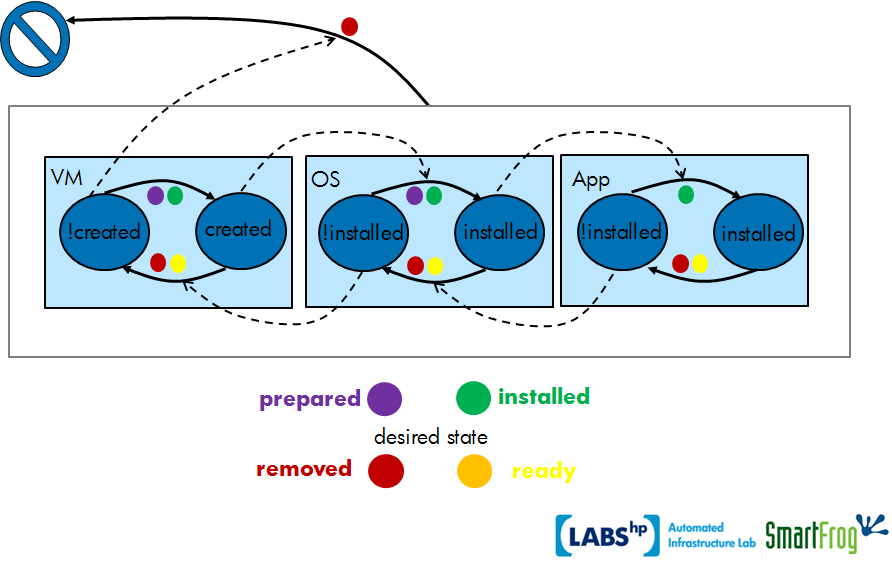
\includegraphics[scale=0.5]{des}
\caption{An Orchestration with Explicit Desired State}\label{Des}
\end{figure}

In the figure, all of the transitions have ``coloured-dot'' dependencies on them.  These indicate necessary conditions related to ``current desired state'' for their enablement. (Some have further conditions too.)  For any of the transitions, one of the coloured desired states must hold for the transition to be enabled.  For instance, for \cd{OS}, the desired state for the composite/model must be \cd{prepared} or \cd{installed} for the transition from \cd{!installed} to \cd{installed} in \cd{OS} to be enabled.  This transition has a further condition, namely that \cd{VM}'s \cd{created} attribute is set to \cd{true}.  

Note also, for interest, that there is a termination condition on the model which holds when the desired state is \cd{removed} and \cd{VM}'s \cd{created} attribute is \cd{false}. 

\subsection*{Representation of State Component Transitions}
Note that for all but the simplest component descriptions, it will \textit{not} be feasible to represent each state of a component individually.  This is because there are potentially significantly many states.  

As a result, what should primarily represented are \textit{transition schemas} between a source \textit{set} of states and a target \textit{set} of states.  Refer to Figure~\ref{Schemas}. 

\begin{figure}[!h]
\centering
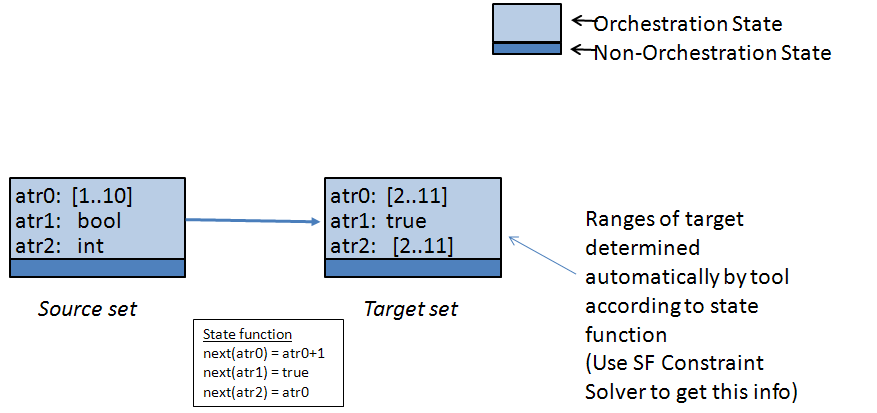
\includegraphics[scale=0.5]{trans}
\caption{A Single Transition Schema within a State Component}\label{Schemas}
\end{figure}

The primary currency for specifying the behaviour of components is thus individual transition schemas, rather than specifying a state machine as a single unit.  Notice from the figure that the source of a transition schema is a set of states -- it does fix precise values for the attributes, which means that the source is not a representation of a single state but rather a set of them.  This holds similarly for the sink/target set of states.  

It should be possible to specify the state functions of a transition schema with the authoring tool, and for the ranges of the attributes in the target set to be derived \textit{automatically} by the tool.  The tool can use the SmartFrog Constraint Solver, for instance, to derive the new ranges of attributes.

It should be feasible for meaningful names to be given to source and target state sets which may aid readability of the model.  Moreover, when the tool recognises that the source set of one transition schema is a subset $\subseteq$ of the sink/target set of another, it may link them visually.  Finally, in degenerative/simple cases, the source and target may correspond to a single state, and if this is the case throughout the model it will be possible to represent the transition schemas (which are now just plain transitions) as a single state machine. 

The \cd{created}/\cd{removed} \cd{ManagedEntity} example which was discussed at the start of this document is an example of a degenerative case where transition schemas are transitions and where the authoring tool should link the transitions together into a single state machine. 

\cleardoublepage
\section{Run-time monitoring}
Run-time monitoring should be enabled, \textit{for example} to:
\begin{itemize}
\item Provide feedback of current state
\item Allow authors/users to turn certain artefacts off/on, such as dependencies or components themselves, say
\item Allow run-time model checking of arbitrary constraints, e.g. so that invariants may be checked (which may not have been guaranteed in the first place)
\item Identify when the current orchestration is deadlocked, save for changes that may be made by asynchronous management logic.

When we check for deadlock in verification, there is still the possibility that no component at some stage of enactment wants to make a transition.  All the deadlock check that we perform at design-time verifies is that some component can always make a transition.  There is a difference here between \textit{can} and \textit{wants}.  The design-time check covers the \textit{can}, a run-time check should cover the \textit{wants}.
\end{itemize}

\cleardoublepage
\section{Local Orchestration -v- Scalable Orchestration}
The current focus of this work sits along the whole spectrum between the extremes of small, very localised orchestrations whose actions are tightly synchronised and large-scale, fault-prone, distributed orchestrations.  For the second of these, it is imperative that components be endowed with sufficient autonomy so that they may perform actions when they deem them appropriate.  This dispensation is at odds with the first enumerated extreme of orchestration, where the performance of actions is prescribed for components as part of some globally synchronised behaviour, where they are forced to be in lock-step with each other.  This highly-synchronised form of orchestration will simply not scale, and is not tolerant to faults such as components disappearing. 

For the time being, at least, we are interested in investigating how we might usefully support applications of orchestration at arbitrary points along the described spectrum.  As a result, we keep an open mind regarding the types of modelling artefacts that we should support in our orchestration language.  It is notable that the current modelling language is very much oriented towards the scalable extreme, but even for this purpose there is much work that could be done in fine tuning our approach.  Our principle interest here is in management orchestrations where there may be potentially tens or hundreds of thousands of components that need managing.  Imposing tightly synchronised behaviour in this context is simply not feasible.  In contrast, we also have applications of orchestration that we are interested in supporting that sit towards the localised extreme.  

\cleardoublepage
\section{Functional Tests}
There are a number of functional tests located at: \cd{org.smartfrog.test.system.dependencies.*}

\cleardoublepage
\bibliographystyle{plain}
\bibliography{SFOrchestration1_2}

\end{document}

